\section{Limitations of Commercial Servos}
\label{sec:limitations}

The initial prototyping phase considered the use of the MG996R \cite{mg996r}, a ubiquitous standard-size
servomotor widely adopted in hobbyist robotics. However, a rigorous characterization revealed fundamental
limitations that rendered these units unsuitable for high-fidelity gait control.

The critical deficiencies, ranked by their impact on system performance, are:

\begin{itemize}
    \item \textbf{Feedback Sensor Degradation:} The internal feedback mechanism relies on a low-cost
        resistive potentiometer. Unlike non-contact solutions, this component involves a physical wiper
        sliding over a resistive track. Continuous operation leads to mechanical wear, causing progressive
        signal degradation and non-linearity. This deterioration was experimentally identified as the
        primary source of long-term positioning error.

    \item \textbf{Deadband and Stick-Slip Behavior:} To prevent motor hunting, the MG996R specifies a dead
        band width of $5\,\mu s$~\cite{mg996r}. When combined with the high static friction (stiction) of
        the metal gear assembly, this results in a significant effective dead-zone, making the joint fail
        to move for small command increments.

    \item \textbf{Limited Control Resolution and Bandwidth:} The standard PWM control protocol is inherently
        limited by the update rate. As per specifications, the MG996R operates on a $20\,ms$ period ($50\,Hz$
        frequency)~\cite{mg996r}. This low update frequency acts as a bottleneck for high-dynamic control loops,
        introducing a delay of up to $20\,ms$ between command and actuation.

    \item \textbf{Manufacturing Variability:} Significant unit-to-unit inconsistency was observed regarding
        the operational range characteristics. Two identical servos receiving the same PWM signal often
        align to different physical angles. This lack of repeatability makes the IK model unreliable without
        an intensive, individual calibration for each joint.

    \item \textbf{Obsolete Open-Loop Architecture:} Finally, as confirmed by the standard 3-pin interface
        (PWM, $V_{cc}$, GND)~\cite{mg996r}, these servos operate as "black boxes". The internal PID
        controller is hard-wired and inaccessible, preventing the implementation of advanced friction
        compensation or different control architectures in general. Crucially, the lack of feedback (current,
        real position, temperature) prevents any form of centralized Hardware-in-the-Loop control or online
        diagnostics.
\end{itemize}

To visualize and confirm the newly introduced limitations, an experimental characterization was performed
on two randomly selected units (Motor A and Motor B). The results, presented in Figure
\ref{fig:servo_deficiencies}, map the control signal pulse width ($T_{on}$) against the actual output
angle measured by a high-precision external magnetic encoder. The test involved a full sweep from $0.5\,ms$
to $2.5\,ms$ (Forward path, blue line) followed by a return to $0.5\,ms$ (Backward path, orange line).

\begin{figure}[htbp]
    \centering
    \begin{subfigure}[b]{0.48\textwidth}
        \centering
        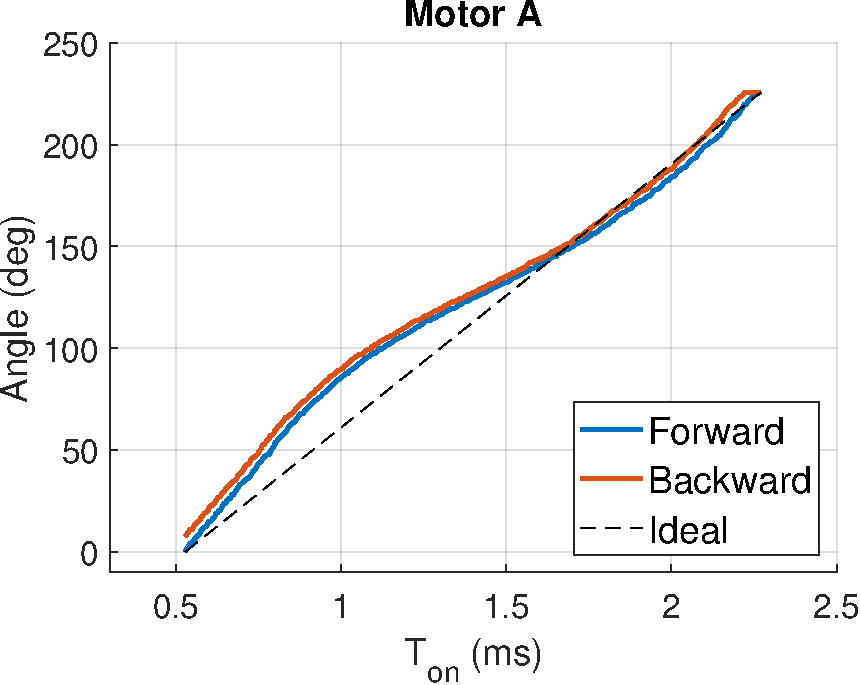
\includegraphics[width=\textwidth]{images/motor_char_A.pdf}
        \caption{}
        \label{fig:motor_A}
    \end{subfigure}
    \hfill
    \begin{subfigure}[b]{0.48\textwidth}
        \centering
        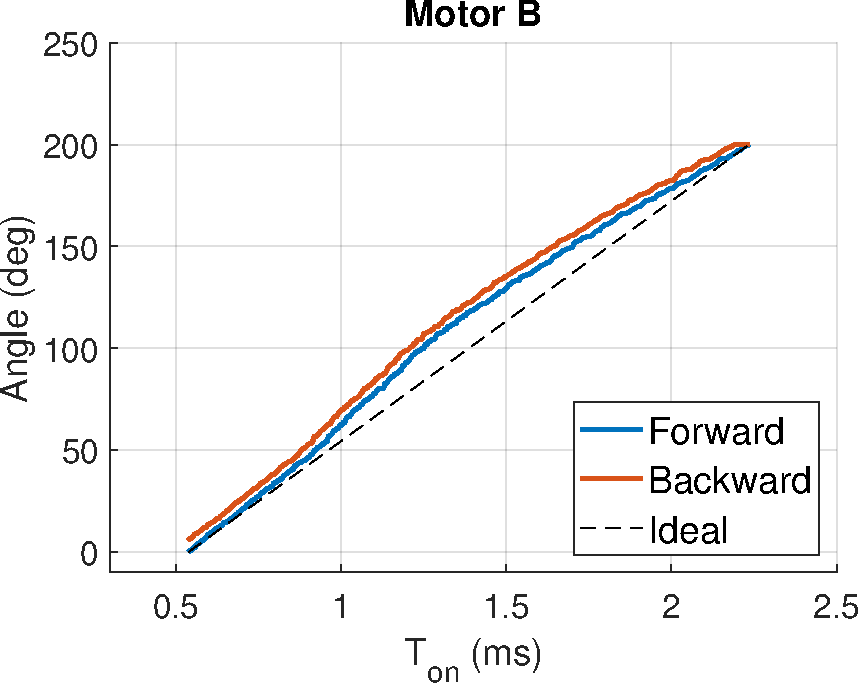
\includegraphics[width=\textwidth]{images/motor_char_B.pdf}
        \caption{}
        \label{fig:motor_B}
    \end{subfigure}
    \caption{Experimental Characterization of two MG996R Units.}
    \label{fig:servo_deficiencies}
\end{figure}

The dashed black line represents the ideal linear response ($Angle \propto T_{on}$) expected from a servomotor,
adjusted for the motor effective operative range. Both units show severe deviations from this ideal behavior,
introducing position errors exceeding $15^{\circ}$ thus making precise open-loop control impossible without a
complex, motor-specific calibration lookup table.

Furthermore, both plots exhibit a considerable hysteresis loop, visible as the vertical gap between the
forward and backward trajectories for the same PWM input.

Perhaps the most critical finding is the discrepancy between the two nominally identical units. Motor A covers
a range of approximately $0^{\circ}$ to $230^{\circ}$, while Motor B, driven by the exact same signal, spans a
smaller range from roughly $0^{\circ}$ to $200^{\circ}$. It should be noted that the graphs have been truncated
at the endpoints where a change in $T_{on}$ failed to produce any change in output position, indicating
mechanical or electronic saturation.

This inconsistencies confirms that a unified kinematic model cannot be applied to a robot using these actuators.
Each joint would require individual characterization and compensation, which is impractical for scalable
deployment.

Finally, although not visible at this macro-scale zoom, the stepped nature of the data acquisition
(confirmed during testing) revealed that the motors often remained stationary for input changes of
$5-10\,\mu s$ (corresponding to $1-2$ PWM step increments @$50\, Hz$), jumping only when the accumulated
error overcame the internal deadband and static friction.

Given these fundamental constraints, simply upgrading to a slightly more expensive hobby servo would yield
diminishing returns. The only viable solution was to redesign the control electronics entirely, retaining only
the mechanical shell and the DC motor, to create a fully programmable, closed-loop actuator.
